\index{Test Case!Replace}
\index{Replace!Test Case}

\app{} lets you \bxname{replace} one or more \gdcases{} in an editor with another \gdcase{} from your library of \gdcases{}. This is useful if you have created a module to replace one or more \gdcases{} and you want to be guided through the replacement process.


\begin{enumerate}
\item Open the \gdtestcaseeditor{} or \gdtestsuiteeditor{} by double-clicking on the \gdcase{} or \gdsuite{} you  want to edit. 
\item Select the \gdcases{} you want to replace by single-clicking them. Use 
  \bxkey{Ctrl} to select more than one item. 
\item Right-click in the editor and  select: \\
\bxmenu{Refactor}{Replace with Test Case}{}.
\item The first page of a wizard appears in which you can replace selected the \gdcases{} in a series of steps. 
\end{enumerate}

\bxwarn{You may only replace single \gdcases{} which neither have multiple data sets nor central test data / Excel files as data.}


\textbf{Page 1: Replacing the \gdcases{}}
\begin{enumerate}
\item On the first page of the wizard \bxfigref{ReplaceTC-ChooseTC}, you can select a  new  \gdcase{} to replace the selected \gdcases{}. 
\item Browse to and select the \gdcase{} you want to add to the editor.
\item Click \bxcaption{Next} to match the component names for the old and new \gdcases{}, or click \bxcaption{Finish} to replace the selected \gdcases{} with the bare new \gdcase{}, without any component names transferred. 
\end{enumerate}

\begin{figure}[h]
\begin{center}
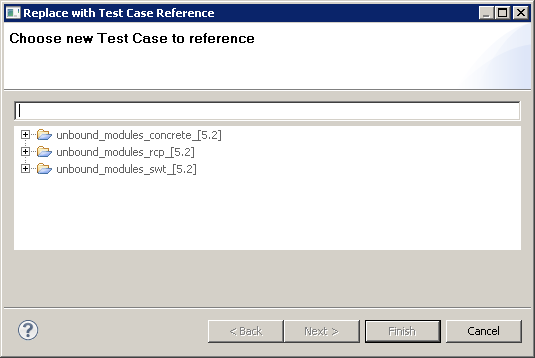
\includegraphics[width=12.5cm]{Tasks/Editors/PS/ReplaceTC_ChooseTC}
\caption{Select \gdcase{}}
\label{ReplaceTC-ChooseTC}
\end{center}
\end{figure} 


\textbf{Page 2: Matching component names}
\begin{enumerate}
\item On the second page of the wizard \bxpref{ReplaceTC-CompNames}, you can see an overview of component names for the replacement. 
\begin{itemize}
\item On the left-hand side you can see any component names that were entered for the \gdcases{} to be replaced. If the component names were propagated \bxpref{TasksCompNamesCheckbox}, you will see a small yellow arrow on the component name icon. 
\bxtipp{If the old \gdcases{} contained no component names, then you will see the text \bxname{no component names}.}
\item On the right-hand side, you can see the \gdcompnamesview{}, which shows any component names that are required by the new \gdcase{}. 
\end{itemize}
\item Use this dialog to transfer any component names from the old \gdcases{} to the new \gdcases{}. You can enter component names, or you can leave the new component names as they are. You can also set the checkbox in the \gdcompnamesview{} to propagate the name to the next \gdcase{} in the hierarchy.  
\item Once you have transferred the component names, you can click \bxcaption{Next} 
%to match parameters, 
to add further information
or you can click \bxcaption{Finish} to replace the selected \gdcases{} with the new \gdcase{} and the selected component names. 
\end{enumerate}

\begin{figure}[h]
\begin{center}
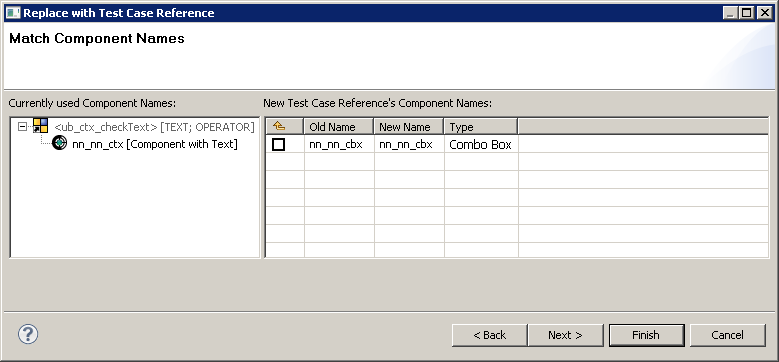
\includegraphics[width=12.5cm]{Tasks/Editors/PS/ReplaceTC_CompNames}
\caption{Match component names}
\label{ReplaceTC-CompNames}
\end{center}
\end{figure} 

%% \textbf{Page 3: Matching parameters}
%% \begin{enumerate}
%% \item On the third page of the wizard, you can see an overview of parameters and data for the replacement.
%% \begin{itemize}
%% \item On the left-hand side you can see any parameters and data that  were entered for the \gdcases{} to be replaced. 
%% \bxtipp{If the old \gdcases{} contained no parameters, then you will see the text \bxname{no parameters}.}
%% \item On the right-hand side, you can see any parameters and data that are required by the new \gdcase{}. 
%% \end{itemize}
%% \item Use this dialog to transfer any parameters from the old \gdcases{} to the new \gdcases{}. 
%% %You can drag and drop old component names onto to new ones, you can enter new component names, or you can leave the new component names as they are. You can also set the checkbox in the \gdcompamesview{} to propagate the name to the next \gdcase{} in the hierarchy.  
%% \item Once you have transferred the parameters, you can click \bxcaption{Next} to enter a \gdcase{} reference name and comment, or you can click \bxcaption{Finish} to replace the selected \gdcases{} with the new \gdcase{} and the selected component names and parameters.
%% \end{enumerate}

\textbf{Page 3: Further information}
\begin{enumerate}
\item On the final page of the wizard, you can enter a \gdcase{} reference name and a comment for the new \gdcase{}. 
\item Once you have entered a name and/or a comment, you can click \bxcaption{Finish} to complete the replacement.
\end{enumerate}


Once you have replaced the \gdcase{}, you must manually adapt the parameters for the new \gdcase{}.
